\section{Filter}
Efter signalet er blevet forstærket skal det filtreres, så alle de uønskede signaler kan dæmpes. Der benyttes kun et lavpasfilter, da det ønskede signal ligger i frekvensområdet 0-12 Hz, (henvisning til blokdiagram/kravspecifikation?). Filtre kan udarbejdes både som et passivt filter og et aktivt filter. Hvis signalet ligger i frekvensområdet under 1 MHz anbefales det at benytte aktive filtre \cite{Op amps for everyone}. Aktiv filtre benytter operationforstærkere, kondensatorer og modstande, hvor et passivt benytter kondensatorer, modstande og spoler \cite{Op amps for everyone}. Der findes flere forskellige typer filter heriblandt et Butterworth filter, et Tschebyschevfiltre og et Besselfilter. Butterworth filteret giver maksimal fladhed i pasbåndet og stopbåndet. Tschebyschevfilteret giver den hurtigste overgang fra pasbåndet til stopbåndet. Besselfilteret giver en lineær faserespons, hvilket vil sige at fasen er lineær med frekvensen.\fxnote{Fasen angiver hvor godt et signals frekvensspektrum bliver gengivet}\fxnote{skal vi have et billede ind af de forskellige typer?} \cite{Op amps for everyone} Butterworthfilteret benyttes til at filtrere dette signal, da der ønskes maksimal fladhed i pasbåndet og stopbåndet.\fxnote{Henvisning til kravspecifikation}

I afsnit (henvisning til kravspecifikation) på side (henvisning) blev karakteristikaene af lavpasfilteret bestemt. Der kræves en minimumsdæmpning af stopbåndet $(Amin)$ på 20 dB, der accepteres en maksimal variation af pasbåndet $(Amax)$ på 3 dB, knækfrekvensen $(\omega _p)$ er på 12 Hz, samt en stopbåndstærskel $( \omega _s)$ på 45 Hz. Nedenfor ses en illustration af hvad de forskellige karakteristka beskriver.

\begin{figure}[H]
\center
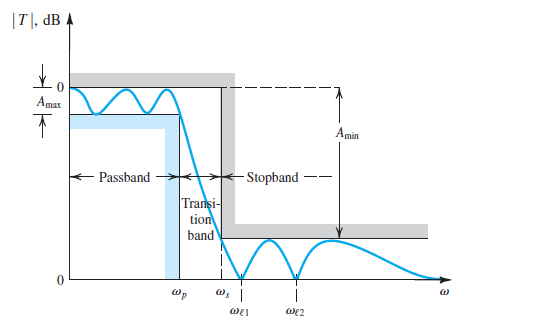
\includegraphics[scale=1]{figures/cProblemloesning/Lavpasfilter_generisk.PNG}
\caption{Figuren viser et bodeplot hvor de fire karakteristika af et lavpasfilter er angivet.}
\label{fig:lavpasfilter_generisk}
\end{figure} 

Ud fra karakteristikaene af filteret kan filterets orden bestemmes ved ligningen: 
\begin{equation} \label{eq:lavpasfilter}
A(\omega _s) = 10 \cdot \left[1 + \epsilon^2 \frac{\omega _s}{\omega _p}^2N\right] 
\end{equation}

I ligning \ref{eq:lavpasfilter} er filterets orden angivet af N, når alle de andre variable kendes kan ordenen udregnes. I ligningen betegner $A(\omega _s)$ den minimale dæmpning der kræves stopbåndet. $\epsilon$ er udtrykt ved ligningen
\begin{equation}
\epsilon = \sqrt{10^A_max/10 - 1}
\end{equation}

\section{Design}
Ordenen af lavpasfilteret bestemmes ved at sætte værdierne fra (henvisning til kravspecifikation) ind i ligningen \ref{eq:lavpasfilter}, udregningen vil se ud som følgende:
\begin{equation}
\epsilon = \sqrt{103dB/10 - 1} = 0.998
\end{equation}
\begin{equation}
20dB = 10 \cdot \left[1 + 0.998^2 \frac{45Hz}{12Hz}^2N\right]
\end{equation}
\begin{equation}
N = 1.74 \approx 2
\end{equation}

Grunden til at ordenen rundes op til 2 er, at filterets orden kun kan angives i hele tal, og hvis kravene til filteret skal overholdes skal der altid rundes opad. 

Der er to forskellige måder at designe et andet ordens lavpasfilter på: Sallen-Key topology og Multiple Feedback topology. Her benyttes Sallen-Key topologien. På figur \ref{fig:SallenKey} ses et 2. ordens lavpasfilter designet efter Sallen-Key topologien.
\begin{figure}[H]
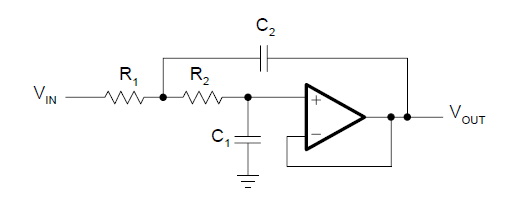
\includegraphics[scale=1]{figures/cProblemloesning/SallenLavpas.PNG}
\caption{Figuren illustrer et andet ordens unity-gain Sallen-Key lavpasfilter}
\label{fig:SallenKey}
\end{figure}
Værdierne for modstandene kan udregnes med følgende ligning:
\begin{equation} \label{eq:LavpasModstande}
R_1,2 = \frac{a_1 C_2 \pm \sqrt{A_1^2 C_2^2 - 4b_1 C_1 C_2}}{4 \pi f_c C_1 C_2}
\end{equation}

For at finde reelle værdier under kvadratroden skal følgende være opfyldt:
\begin{equation} \label{eq:kondensator}
C_2 \geq C_1 \frac{4b_1}{a_1^2}
\end{equation}

I ligning \ref{eq:LavpasModstande} står C variablene for kondensatorer, R variablene står for modstande, $a_1$ og $b_1$ er konstanter, mens $f_c$ er den valgte knækfrekvens. 

For at udregne modstandene vælges $C_1$ til at være 100nF, ud fra dette kan $C_1$ bestemmes med ligning \ref{eq:kondensator}:
\begin{equation}
C_2 \geq 100nF \frac{4\cdot 1}{1.4142^2} = C_2 \geq 200nF
\end{equation}

Ud fra ovenstående ligning vælges $C_2$ til at være 480nF, dermed kan $R_1$ og $R_2$ beregnes med ligning \ref{eq:LavpasModstande}:
\begin{equation}
R_1,2 = \frac{1.4142 \cdot 480nF \pm \sqrt{1.4142^2 480nF^2 - 4 \cdot 1 \cdot 100nF \cdot 480nF}}{4 \pi 12Hz 100nF 480nF} = 16540, 2215.53
\end{equation}

